
	\chapter{RESULTS \& DISCUSSION}
	\label{chap:results}
		In this chapter the inclusion of EVs and its impact of power loss in the presence of loads in the system is analyzed.
		

		
		
		
	\section{Simulation Outputs}
	The datas given below are about the Most Economic Time interval to Charge the Vehicle, charging Patterns and Voltage magnitude graphs for different scenarios.
			\subsection{Charging Patterns}
	These plots depict the charging and discharging pattern for the classified vehicles. 216 vehicles are taken into consideration for each vehicle type and the charging pattern is identified.
	
	
	
	\begin{figure}[!h]
		\centering
		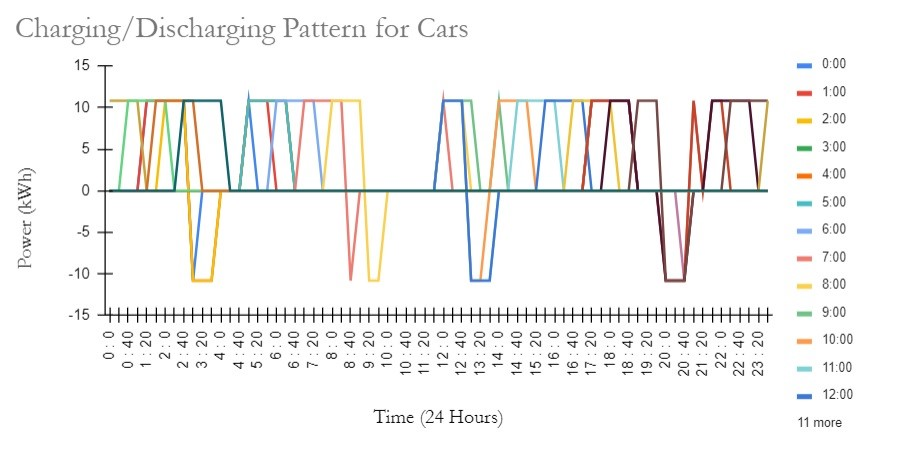
\includegraphics[width=0.7\linewidth]{Figures/cp_case1}
		\caption{Charging/Discharging pattern for Cars}
		\label{fig:cpcase1}
	\end{figure}
	
	\begin{figure}[!h]
		\centering
		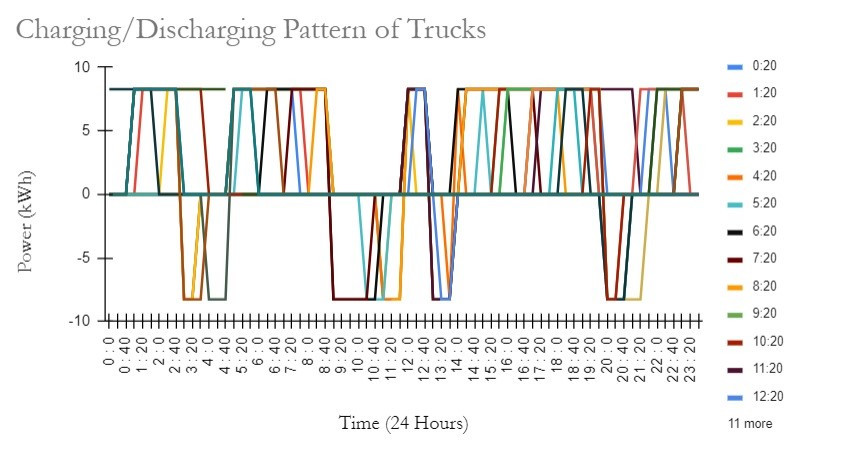
\includegraphics[width=0.7\linewidth]{Figures/cp_case2}
		\caption{Charging/Discharging pattern for Trucks}
		\label{fig:cpcase2}
	\end{figure}
	
	\begin{figure}[!h]
		\centering
		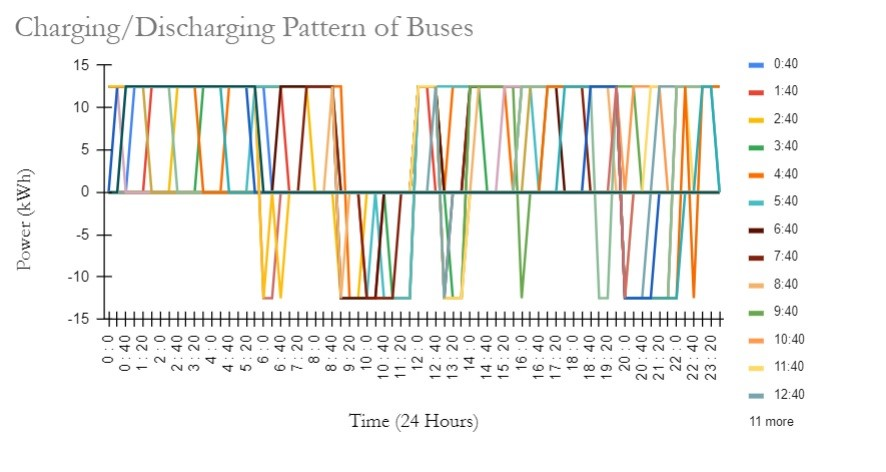
\includegraphics[width=0.7\linewidth]{Figures/cp_case3}
		\caption{Charging/Discharging pattern for Buses}
		\label{fig:cpcase3}
	\end{figure}
	
	\noindent A strategic pattern is established to maintain the stability of the grid by comparing the vehicle capacity to the Real time price for each hour. When the price is low, the vehicle is put to charge and when the price is high,the vehicle is put to discharge in comparision with the peak demand. By this way the overall cost is drastically reduced , leading to profit for the user and at the same time the overall load in the grid decreases making the load demand curve flatter.
	
	
		\subsection{Economic Charging}
		
			Three cases are taken in this study which are namely:
				\newline Case 1(00:00): Case 1 depicts that the vehicles has Started on a hourly basis i.e. the 1 hour block.
				\newline Case 2(00:20) : Case 2 depicts that the vehicle has Started from the 20th min of an hour i.e. 20mins block.
				\newline Case 3(00:40): Case 3 depicts that the vehicles has Started from the 40th minute of an hour i.e. 40th minute block
			
			\begin{table}[!h]
				\caption{Most Economic Time interval to Charge the Vehicle}
				\centering
			\begin{tabular}{|l|l|l|l|}
				\hline
				\textbf{VEHICLE TYPE}           & \textbf{CASE}         & \textbf{BEST PRICE} & \textbf{HOUR} \\ \hline
				\multirow{3}{*}{\textbf{CAR}}   & \textbf{Case 1 - (00:00)} & - \$1.71            & 12:00         \\ \cline{2-4} 
				& \textbf{Case 2 - (00:20)} & - \$2.09            & 01:20         \\ \cline{2-4} 
				& \textbf{Case 3 - (00:40)} & - \$1.58            & 01:40         \\ \hline
				\multirow{3}{*}{\textbf{BUS}}   & \textbf{Case 1 - (00:00)} & - \$0.47            & 12:00         \\ \cline{2-4} 
				& \textbf{Case 2 - (00:20)} & - \$1.25            & 20:20         \\ \cline{2-4} 
				& \textbf{Case 3 - (00:40)} & - \$0.69            & 11:40         \\ \hline
				\multirow{3}{*}{\textbf{TRUCK}} & \textbf{Case 1 - (00:00)} & - \$2.57            & 05:00         \\ \cline{2-4} 
				& \textbf{Case 2 - (00:20)} & -\$1.00             & 04:20         \\ \cline{2-4} 
				& \textbf{Case 3 - (00:40)} & - \$2.11            & 04:40         \\ \hline
			\end{tabular}
		\label{table:ec}
		\end{table}
		
		

	%\subsection{Maximum EV Load}
	
		In the table \ref{table:whichbus} the hour at which the maximum load is present is shown for Scenario-1 and Scenario-2 along with the load present in the system.
		
			\begin{table}[!h]
			\centering
			\caption{Hour at which the EV Load is maximum }
			\begin{tabular}{|ll|ll|ll|ll|}
				\hline
				\multicolumn{2}{|l|}{\textbf{Scenario}} & \multicolumn{2}{l|}{\textbf{Case-1}} & \multicolumn{2}{l|}{\textbf{Case-2}} & \multicolumn{2}{l|}{\textbf{Case-3}} \\ \hline
				\multicolumn{2}{|l|}{\textbf{Scenario-1}}        & \multicolumn{2}{l|}{$ 19^{th} $}            & \multicolumn{2}{l|}{$ 6^{th} $}             & \multicolumn{2}{l|}{$ 19^{th} $}             \\ \hline
				\multicolumn{2}{|l|}{\textbf{Scenario-2}}        & \multicolumn{2}{l|}{$ 13^{th} $}           & \multicolumn{2}{l|}{$ 6^{th} $}             & \multicolumn{2}{l|}{$ 13^{th} $}             \\ \hline
			\end{tabular}
			\label{table:whichbus}
		\end{table}
	

	
	\section{33 bus system}
		In the 33 bus system the EVs are placed at buses 2 (Strongest Bus) and 18 (Weakest Bus) with Voltage Stability Index as a consideration \cite{33bus} .
 		In the provided table \ref{table:powerloss} the power losses are calculated for the corresponding time blocks  as shown in table \ref{table:whichbus} along with the available loads for that particular hour. The results are tabulated in \ref{table:powerloss}.
 		The voltage magnitude of the base case and each time block for  all the cases are computed. Load flow analysis is done on Bus number 2 and Bus number 18 as these are considered to be the best case and worst case buses to calculate the voltage magnitude as referred from \cite{33bus}. From the results it is evident that the loss difference in the grid without EVs connected to the grid(base case) and with EVs connected to the grid on bus number 2 are comparatively lesser. The same loss difference is higher when the EVs connected in 18th bus is high. Looking into voltage magnitude the value of voltage magnitude in base case and EVs connected to the grid on 2nd bus are equal. Whereas in 18th bus it is clear that voltage magnitude when compared to base case is high.
 		
 		\noindent Here figures (\ref{fig:LFa}), (\ref{fig:LFb}) and  (\ref{fig:LFc}) shows the voltage magnitude plot when the EVs are connected to bus 2 and bus 18 during various cases.
 		
 		\noindent and figures (\ref{fig:LF2a}), (\ref{fig:LF2b}) and  (\ref{fig:LF2c}) shows the voltage magnitude plot when the EVs are connected to bus 2 and bus 18 during various cases.
 		
 		
 		
 		
 		
 		\noindent The base case power loss of the 33 bus system is 202.691 `$kWh$' i.e. when the load demand is 100 percent. The summation of all 72 individual loads of cars, trucks and buses for each case is calculated. These additive loads are identified in each time block and the maximum of it is taken into calculation for load flow.

 		\textbf{Case 1:}
 			\begin{itemize}
 				\item Case one is the hourly connection of vehicles starting at 00:00 and the peak load of EVs is found at $19^{th}$ hour with a load of 284.97 $kW$ 
 				\item This load is connected in bus 2 and bus 18 under two different scenarios with active load demand 1 and 0.94 respectively.
 				\item The resulting power loss is 204.104 $kW$ and 253.746 $kW$ respectively for scenario 1 and 189.833 $kW$ and 236.912 $kW$ respectively for scenario 2.
 				\item This shows a 24.49 percent higher loss in scenario 1 and 10.54 percent higher loss in scenario 2.
 			\end{itemize}

 		\textbf{Case 2:}
 		\begin{itemize}
 			\item Case two is the hourly  connection of vehicles starting at 00:20 and the peak load of EVs is found at $6^{th}$ hour with a load of 276.703 $kW$ 
 			\item This load is connected in bus 2 and bus 18 under two different scenarios with active load demand 0.173913043 and 0.83 respectively.
 			\item The resulting power loss is 65.773 $kW$ and 78.460 $kW$ respectively for scenario 1 and 178.967 $kW$ and 222.468 $kW$ respectively for scenario 2.
 			\item This shows a 6.26 percent higher loss in scenario 1 and 1.943 percent higher loss in scenario 2.
 		\end{itemize}
 		
 		\textbf{Case 3:}
 		\begin{itemize}
 			\item Case three is the hourly connection of vehicles starting at 00:40 and the peak load of EVs is found at $19^{th}$ hour with a load of 284.97 $kW$ 
 			\item This load is connected in bus 2 and bus 18 under two different scenarios with active load demand 1 and 0.94 respectively.
 			\item The resulting power loss is 204.104 $kW$ and 253.746 $kW$ respectively for scenario 1 and 189.833 $kW$ and 236.912 $kW$ respectively for scenario 2.
 			\item This shows a 24.49 percent higher loss in scenario 1 and 10.54 percent higher loss in scenario 2.
 		\end{itemize}
 		
 		From the figure \ref{fig:loadprofile33},  we can identify that the difference in voltage magnitudes differ highly from the base case on the $18^{th}$ bus and remains almost constant on the $2^{nd}$ bus, this concludes that Bus 18 is the weakest bus and Bus 2 isthe strongest bus in this 33 bus system. 
 		
 		
 		
 		
 		
 		
 		
 		
 		
 		
 		
 		
 		
 		
 		
 				\begin{table}[!t]
 			\centering
 			\caption{Power Loss when EV is connected in a 33 bus system}
 			\begin{tabular}{|c|c|cc|cc|cc|}
 				\hline
 				\multirow{2}{*}{\textbf{Scenario}}                            & \multirow{2}{*}{\textbf{\begin{tabular}[c]{@{}c@{}}Base\\ Case\\ Power\\ Loss\\ (kW)\end{tabular}}} & \multicolumn{2}{c|}{\textbf{Case 1}}                                                                                                                                                                          & \multicolumn{2}{c|}{\textbf{Case 2}}                                                                                                                                                                          & \multicolumn{2}{c|}{\textbf{Case 3}}                                                                                                                                                                          \\ \cline{3-8} 
 				&                                                                                              & \multicolumn{1}{c|}{\textbf{\begin{tabular}[c]{@{}c@{}}Power \\ Loss\\ when EV\\ in Bus 2\\ (kW)\end{tabular}}} & \textbf{\begin{tabular}[c]{@{}c@{}}Power \\ Loss\\ when EV\\ in Bus 18\\ (kW)\end{tabular}} & \multicolumn{1}{c|}{\textbf{\begin{tabular}[c]{@{}c@{}}Power \\ Loss\\ when EV\\ in Bus 2\\ (kW)\end{tabular}}} & \textbf{\begin{tabular}[c]{@{}c@{}}Power \\ Loss\\ when EV\\ in Bus 18\\ (kW)\end{tabular}} & \multicolumn{1}{c|}{\textbf{\begin{tabular}[c]{@{}c@{}}Power\\  Loss\\ when EV\\ in Bus 2\\ (kW)\end{tabular}}} & \textbf{\begin{tabular}[c]{@{}c@{}}Power \\ Loss\\ when EV\\ in Bus 18\\ (kW)\end{tabular}} \\ \hline
 				\textbf{\begin{tabular}[c]{@{}c@{}}Scenario\\ 1\end{tabular}} & \multirow{2}{*}{202.691}                                                                     & \multicolumn{1}{c|}{204.104}                                                                                    & 253.746                                                                                     & \multicolumn{1}{c|}{65.773}                                                                                     & 78.460                                                                                      & \multicolumn{1}{c|}{204.104}                                                                                    & 253.746                                                                                     \\ \cline{1-1} \cline{3-8} 
 				\textbf{\begin{tabular}[c]{@{}c@{}}Scenario\\ 2\end{tabular}} &                                                                                              & \multicolumn{1}{c|}{189.833}                                                                                    & 236.912                                                                                     & \multicolumn{1}{c|}{178.967}                                                                                    & 222.468                                                                                     & \multicolumn{1}{c|}{189.833}                                                                                    & 236.912                                                                                     \\ \hline
 			\end{tabular}
 			\label{table:powerloss}
 		\end{table}
 	
 		\begin{figure}[!h]
 			\begin{subfigure}{.5\textwidth}
 				\centering
 				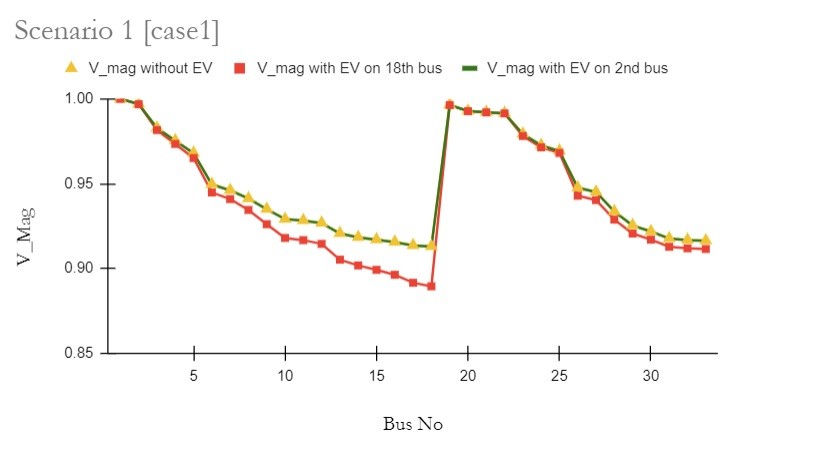
\includegraphics[width=.97\linewidth,height= 4.95cm]{./Figures/sc1_case1}  
 				\caption{Case I}
 				\label{fig:LFa}
 			\end{subfigure}
 			\begin{subfigure}{.5\textwidth}
 				\centering
 				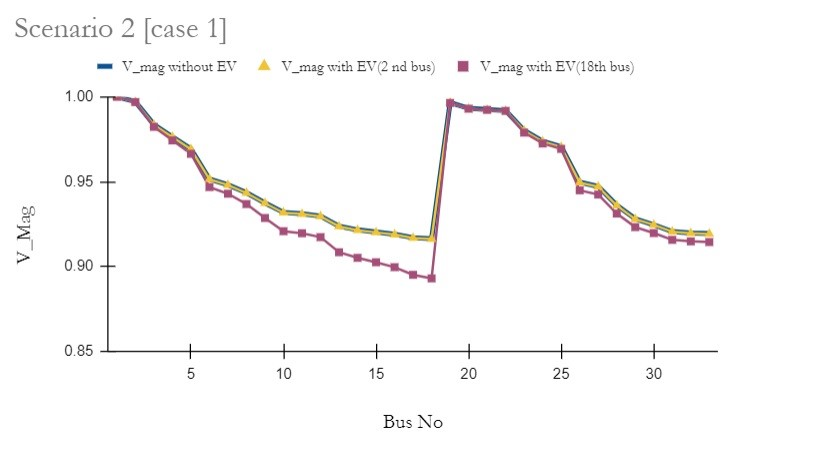
\includegraphics[width=.97\linewidth,height= 4.95cm]{./Figures/sc2_case1}  
 				\caption{Case I}
 				\label{fig:LF2a}
 			\end{subfigure}
 			\begin{subfigure}{.5\textwidth}
 				\centering
 				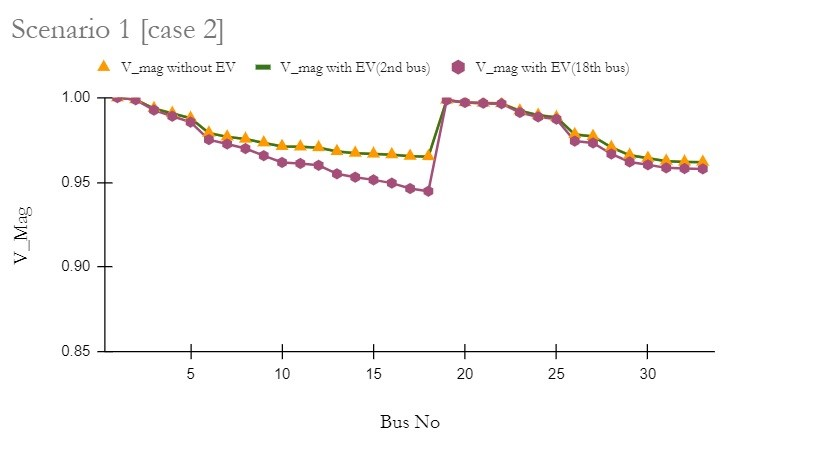
\includegraphics[width=.97\linewidth,height= 4.95cm]{./Figures/sc1_case2}
 				\caption{Case II}
 				\label{fig:LFb}
 			\end{subfigure}
 			\begin{subfigure}{.5\textwidth}
 				\centering
 				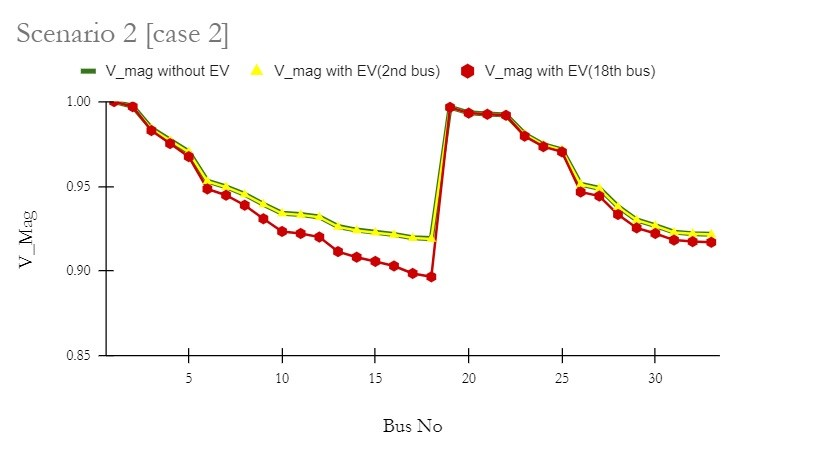
\includegraphics[width=.97\linewidth,height= 4.95cm]{./Figures/sc2_case2}
 				\caption{Case II}
 				\label{fig:LF2b}
 			\end{subfigure}
 			\begin{subfigure}{.5\textwidth}
 				\centering
 				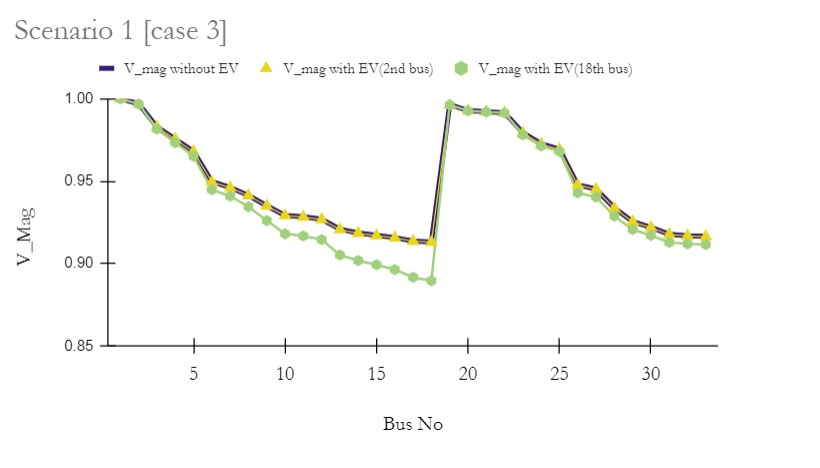
\includegraphics[width=.97\linewidth,height= 4.95cm]{./Figures/sc1_case3}
 				\caption{Case III}
 				\label{fig:LFc}
 			\end{subfigure}
 			\begin{subfigure}{.5\textwidth}
 				\centering
 				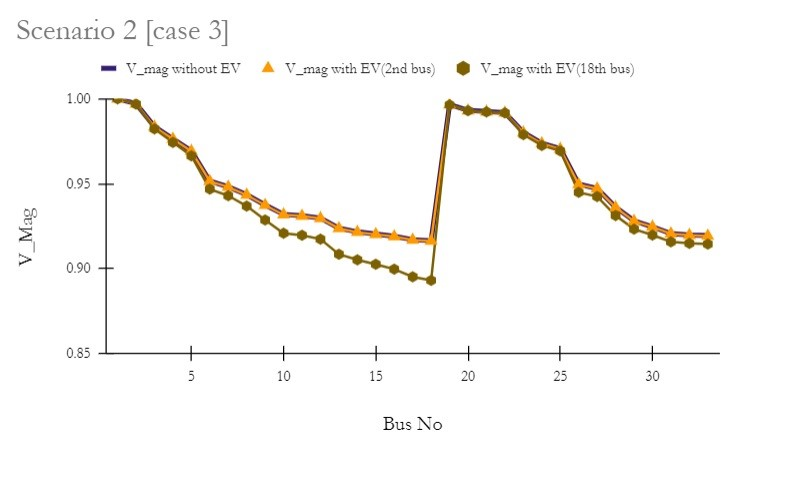
\includegraphics[width=.97\linewidth,height= 4.95cm]{./Figures/sc2_case3}
 				\caption{Case III}
 				\label{fig:LF2c}
 			\end{subfigure}
 			\caption{ Voltage magnitude variation for different scenarios on 33 bus system }
 			\label{fig:loadprofile33}
 		\end{figure} 
 		
		
	



	\section{69 bus system}
In the provided table \ref{table:powerloss69} the power loss is calculated in such a way that the time blocks having the maximum load  is considered and then load flow analysis is performed on 2nd bus(best case)and 54th bus (worst case) of 69 bus system to find the variation of load with and without EV .


\begin{table}[!h]
				\centering
	\caption{Power Loss when EV is connected in a 69 bus system}
	\begin{tabular}{|c|c|cc|cc|cc|}
		\hline
		\multirow{2}{*}{\textbf{Scenario}}                            & \multirow{2}{*}{\textbf{\begin{tabular}[c]{@{}c@{}}Base\\ Case\\ Power\\ Loss\\ (kW)\end{tabular}}} & \multicolumn{2}{c|}{\textbf{Case 1}}                                                                                                                                                                          & \multicolumn{2}{c|}{\textbf{Case 2}}                                                                                                                                                                          & \multicolumn{2}{c|}{\textbf{Case 3}}                                                                                                                                                                          \\ \cline{3-8} 
		&                                                                                              & \multicolumn{1}{c|}{\textbf{\begin{tabular}[c]{@{}c@{}}Power \\ Loss\\ when EV\\ in Bus 2\\ (kW)\end{tabular}}} & \textbf{\begin{tabular}[c]{@{}c@{}}Power \\ Loss\\ when EV\\ in Bus 54\\ (kW)\end{tabular}} & \multicolumn{1}{c|}{\textbf{\begin{tabular}[c]{@{}c@{}}Power \\ Loss\\ when EV\\ in Bus 2\\ (kW)\end{tabular}}} & \textbf{\begin{tabular}[c]{@{}c@{}}Power \\ Loss\\ when EV\\ in Bus 54\\ (kW)\end{tabular}} & \multicolumn{1}{c|}{\textbf{\begin{tabular}[c]{@{}c@{}}Power\\  Loss\\ when EV\\ in Bus 2\\ (kW)\end{tabular}}} & \textbf{\begin{tabular}[c]{@{}c@{}}Power \\ Loss\\ when EV\\ in Bus 54\\ (kW)\end{tabular}} \\ \hline
		\textbf{\begin{tabular}[c]{@{}c@{}}Scenario\\ 1\end{tabular}} & \multirow{2}{*}{226.28}                                                                      & \multicolumn{1}{c|}{207.402}                                                                                    & 220.681                                                                                     & \multicolumn{1}{c|}{198.458}                                                                                      & 210.909                                                                                     & \multicolumn{1}{c|}{207.402}                                                                                    & 220.681                                                                                     \\ \cline{1-1} \cline{3-8} 
		\textbf{\begin{tabular}[c]{@{}c@{}}Scenario\\ 2\end{tabular}} &                                                                                              & \multicolumn{1}{c|}{134.758}                                                                                    & 144.014                                                                                     & \multicolumn{1}{c|}{77.01}                                                                                    & 77.1223                                                                                     & \multicolumn{1}{c|}{134.758}                                                                                    & 144.014                                                                                     \\ \hline
	\end{tabular}
	\label{table:powerloss69}
\end{table}


The voltage magnitude of the base case and each time block for  all the cases are computed. Load flow analysis is done on Bus number 2 and Bus number 54 as these are considered to be the best case and worst case buses to calculate the voltage magnitude as referred from \cite{base}. From the results it is evident that the loss difference in the grid without EVs connected to the grid(base case) and with EVs connected to the grid on bus number 2 are comparatively lesser. The same loss difference is higher when the EVs connected in 54th bus is high. Looking into voltage magnitude the value of voltage magnitude in base case and EVs connected to the grid on 2nd bus are equal. Whereas in 18th bus it is clear that voltage magnitude when compared to base case is high.

\noindent Here figures (\ref{fig:RFa}), (\ref{fig:RFb}) and  (\ref{fig:RFc}) shows the voltage magnitude plot when the EVs are connected to bus 2 and bus 18 during various cases.

\noindent and figures (\ref{fig:RF2a}), (\ref{fig:RF2b}) and  (\ref{fig:RF2c}) shows the voltage magnitude plot when the EVs are connected to bus 2 and bus 18 during various cases.

\begin{figure}[!h]
	\begin{subfigure}{.5\textwidth}
		\centering
		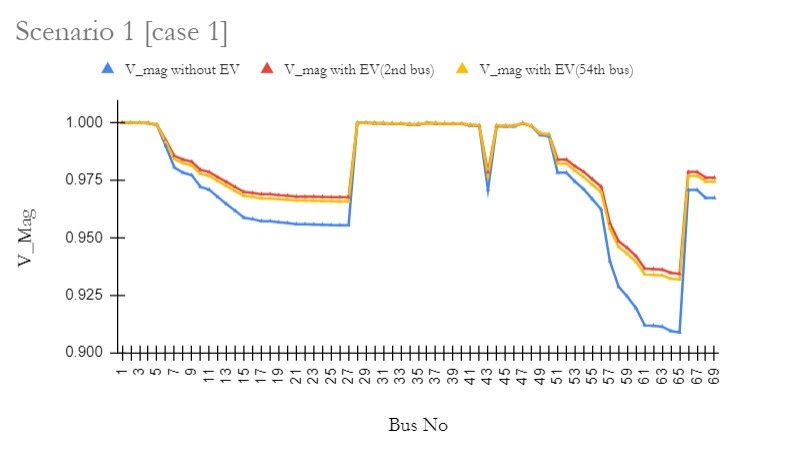
\includegraphics[width=.97\linewidth,height= 4.95cm]{./Figures/69_sc1_case1}  
		\caption{Case I}
		\label{fig:RFa}
	\end{subfigure}
	\begin{subfigure}{.5\textwidth}
		\centering
		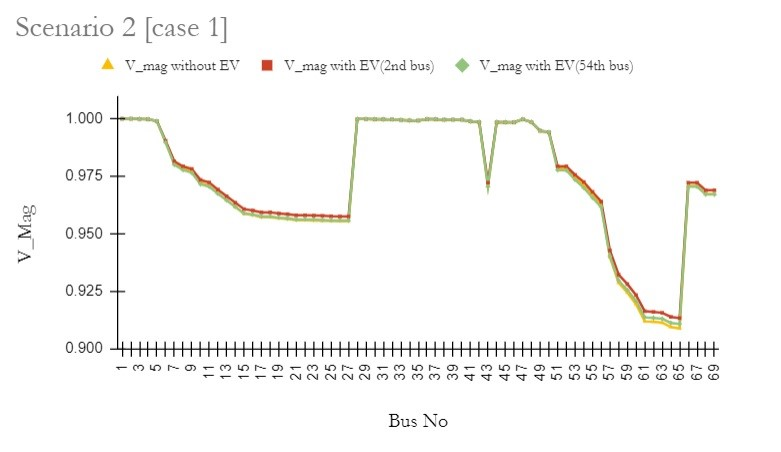
\includegraphics[width=.97\linewidth,height= 4.95cm]{./Figures/69_sc2_case1}  
		\caption{Case I}
		\label{fig:RF2a}
	\end{subfigure}
	\begin{subfigure}{.5\textwidth}
		\centering
		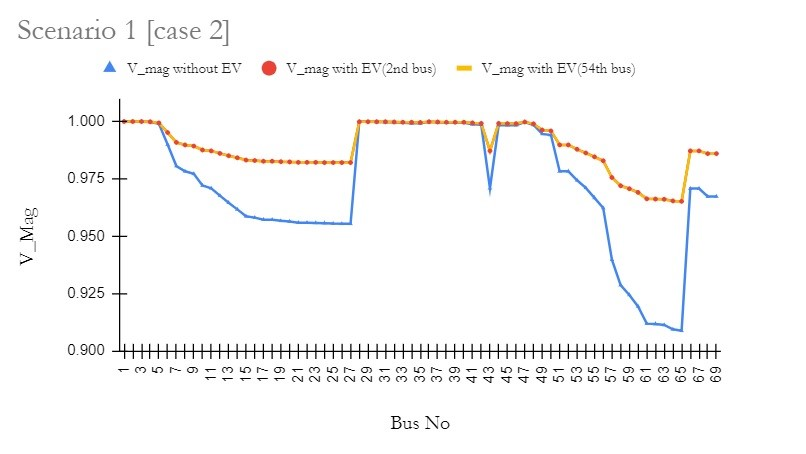
\includegraphics[width=.97\linewidth,height= 4.95cm]{./Figures/69_sc1_case2}
		\caption{Case II}
		\label{fig:RFb}
	\end{subfigure}
	\begin{subfigure}{.5\textwidth}
		\centering
		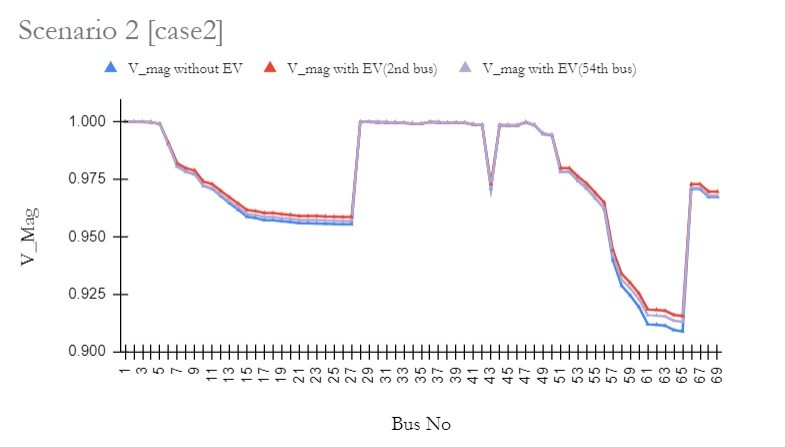
\includegraphics[width=.97\linewidth,height= 4.95cm]{./Figures/69_sc2_case2}
		\caption{Case II}
		\label{fig:RF2b}
	\end{subfigure}
	\begin{subfigure}{.5\textwidth}
		\centering
		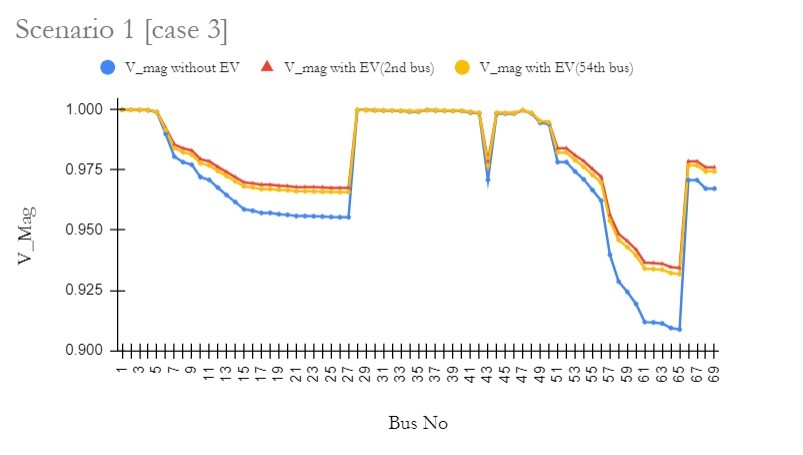
\includegraphics[width=.97\linewidth,height= 4.95cm]{./Figures/69_sc1_case3}
		\caption{Case III}
		\label{fig:RFc}
	\end{subfigure}
	\begin{subfigure}{.5\textwidth}
		\centering
		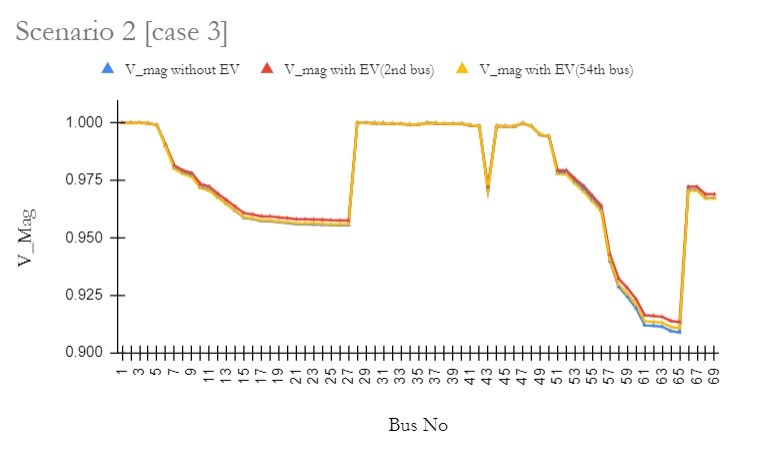
\includegraphics[width=.97\linewidth,height= 4.95cm]{./Figures/69_sc2_case3}
		\caption{Case III}
		\label{fig:RF2c}
	\end{subfigure}
	\caption{ Voltage magnitude variation for different scenarios on 69 bus system  }
	\label{fig:loadprofile69}
\end{figure} 
	
	


		
	
	
	